The program was implemented in Matlab. It consists of one main function that accepts an RGB image as its only input variable, and returns the number corresponding to the correct face in the image database, if found. If however no match is found or the difference between the candidate image and the image stored in the database is to high, the program returns zero.

Initially, the images are color-corrected using the gray world-assumption method. The largest RGB value was detected and used to normalize every channel. The image’s color-space was then converted to YCbCr using Matlab’s built-in function. The chroma channels of the image were then transformed through an implementation of the methods and equations described above. When the chroma channels had been transformed, the mask for the face as well as the mouth and eye map was retrieved as described above. Between each step in the progress, the values were normalized to ensure that precision loss was minimal when values were rounded.

After completing the steps for retrieving eyes and mouth a triangle between the two eyes and the mouth was formed. To do this each eye centroid and mouth centroid was saved in two separate lists. The system then evaluated each mouth centroid with two eye centroids and gave this combination a score based on the assumptions that

\begin{itemize}
  \item eye centroids must be above mouth centroid,
  \item less difference in height of the eye centroids are preferred and
  \item equal distance from the eye centroids to the mouth centroid was preferred.
\end{itemize}

The combinations were then sorted after the sum of these scores in ascending order and the first combination was the proposed face. 

This helps later on to normalize all faces by performing a rotation of the faces. This was done by using Matlabs built in imwarp function. The pivot points for the imwarp were the left and right eye as well as the mouth. The threshold value of the masks was set to be adaptive and decrease if the system could not find a mouth or two sets of eyes.

In order to then further normalize the face, histogram equalization was used to make sure all images had a somewhat even illumination. The result of this equalization can be seen below in figure \ref{fig:withhist}.

\begin{Figure}
  % center it!
  \centering
    % adjust width as you like, include image from optional folder
    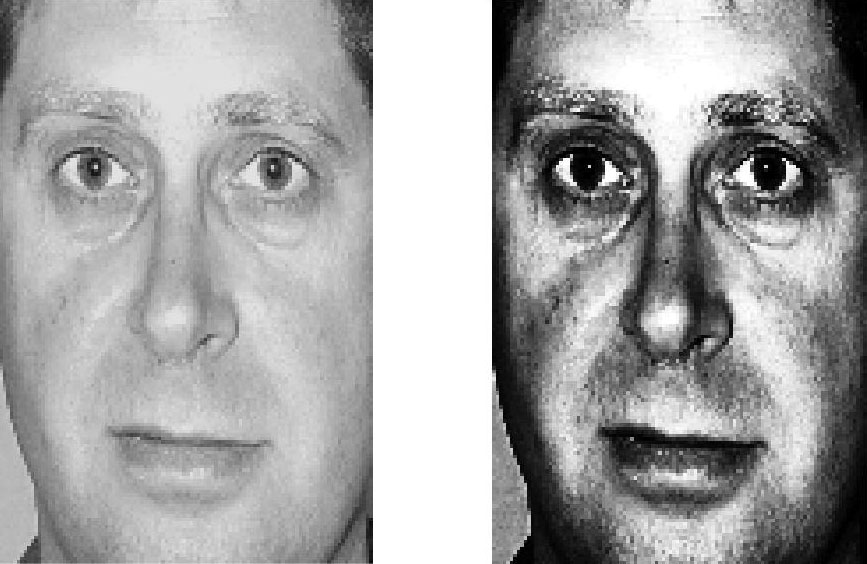
\includegraphics[width=0.7\linewidth]{withhist.jpg}
    % caption! change the label ref to what you want
    \captionof{figure}{\emph{Before and after histogram equalization}\label{fig:withhist}}
\end{Figure}

To create the database, each normalized image were reshaped to a single vector and all images were then stored in a matrix with each row being an image. The PCA of this matrix was performed with Matlab’s Single value decomposition function to retrieve the Eigenfaces sorted in ascending order of the Eigenvalue. The dot product of each normalized image and each Eigenfaces would result in weight values. These values describe how much an Eigenface contributed to recreate the image. The Eigenfaces and the weight values was stored to be used during the recognition process.

When an image was to be recognized, the Eigenfaces’ weight values was retrieved from the image, a process that is described above. When the values for the candidate image had been calculated, the error for each image in the reference database of Eigenface values were calculated using the euclidian distance. The ID of the image in the reference database that had the smallest euclidian error compared to the candidate image gets returned if the error also passed the threshold of the maximum allowed error. This threshold value was found by taking the mean value of the error from all the false positives that the system returned during testing. This ID was what the program returned.
